\chapter{\IfLanguageName{dutch}{Stand van zaken}{State of the art}}%
\label{ch:stand-van-zaken}

% Tip: Begin elk hoofdstuk met een paragraaf inleiding die beschrijft hoe
% dit hoofdstuk past binnen het geheel van de bachelorproef. Geef in het
% bijzonder aan wat de link is met het vorige en volgende hoofdstuk.

% Pas na deze inleidende paragraaf komt de eerste sectiehoofding.

In dit hoofdstuk zal de literatuurstudie besproken worden. Door deze literatuurstudie is het mogelijk om een beter inzicht te krijgen in de technologie en mogelijkheden voor de documentatie van Python projecten. 
Alsook hoe het toegepast kan worden met behulp van Large Language Modellen. Er
zal nadruk worden gelegd op bestaande literatuur en onderzoeken die verbonden
zijn met documentatie van Python projecten. In dit onderdeel zullen verschillende hoofdstukken worden aangekaart. 
Als eerste zal er duidelijk gemaakt worden wat er juist verstaan wordt met documentatie. 
%Ook zal er gekeken worden naar Large Language Modellen
% hoe Solid geïmplementeerd kan worden. Ten slotte zal er ook aandacht worden
% besteed aan vergelijkbare technologieën en aan Europa’s eerste bedrijfsklare Solid
% platform.

\section{Wat is documentatie?}
\label{sec:wat-is-documentatie}

Voor dat er dieper op het onderwerp wordt ingegaan is het belangrijk dat er een duidelijk beeld is van wat documentatie is. 
Waarom is documentatie belangrijk voor een project en wat wordt er begrepen onder documentatie? 

Documentatie is het proces van het vastleggen van de werking van een project.
Dit kan op verschillende manieren gebeuren. 
Er kan gekozen worden om de documentatie te schrijven in de vorm van een handleiding, een wiki, een website of in de vorm van commentaar in de code.
Het doel van documentatie is om de werking van het project te beschrijven zodat andere programmeurs het project kunnen begrijpen en gebruiken.
Zodat er geen tijd verloren gaat aan het lezen van de code en het begrijpen ervan.

Documentatie kan gemaakt worden voor verschillende doelgroepen. Het kan voor interne of externe doeleinden zijn.
Interne documentatie is voor documentatie binnen hetzelfde bedrijf.
Dit gaat dan om het capteren van de process kennis die vergaard is binnen een project, dit is informatie zoals een roadmap of product requirements. 
Of het gaat over het vastleggen van gedetaileerde uitleg over hoe iets werkt en hoe het onderhouden kan worden.

Externe documentatie is voor documentatie die gedeeld wordt met andere bedrijven of klanten. 
Dit gaat dan over de basis werking van de code van een project zodat andere programmeurs het kunnen gebruiken.
Gebruiksaanwijzingen of handleidingen zijn ook een vorm van externe documentatie. \autocite{swimm.io2024}

Voor deze bachelorproef wordt er gekeken naar het documenteren van een Python project.
In de vorm van commentaar in de code en het genereren van een samenvattend document van het gehele project.
Waaruit de werking van het project duidelijk wordt en de relatie tussen de verschillende bestanden en functies.

\section{Wat zijn Large Language Models?}
\label{sec:wat-zijn-llms}

Omdat er in deze bachelorproef gebruik gemaakt wordt van Large Language Modellen is het belangrijk dat er een duidelijk beeld is van wat deze modellen zijn.
En wat deze modellen kunnen, wat de mogelijke beperkingen zijn en wat de huidige stand van zaken is. 
Bestaan er LLMs speciaal getraind op Python code? Kunnen LLMs gebruikt worden om documentatie te genereren? 
Dit zijn enkele vragen die in dit hoofdstuk beantwoord zullen worden. 

Large Language Modellen (LLM) zijn neurale netwerken die getraind worden op grote hoeveelheden tekst. 
Deze modellen kunnen tekst genereren op basis van een gegeven input. 
LLMs hebben een grote vooruitgang gekend in 2017 door de paper van \textcite{VaswaniEtAl2017}. 
Hieruit kwam een nieuw mechanisme transformers dat gebruik maakt van Self-Attention. 
Het gebruik van deze mechanismen zorgde ervoor dat de LLMs beter presteerden op verschillende taken zoals: vertalen, samenvatten, vragen beantwoorden en tekst genereren.

\subsection{{Transformers en Self-Attention}}
\label{sec:transformers-en-self-attention}
Self-Attention duidt dynamisch gewichten toe aan verschillende elementen binnen de meegegeven sequentie, bijvoorbeeld woorden in een zin.
Dit laat het model toe om zich te concentreren op de meest relevante delen van de invoer, terwijl de invloed van minder cruciale delen wordt verminderd.
De invoersequentie wordt eerst in drie verschillende vectoren omgezet: query, key en value.
De Query vector stelt een specifiek token uit de invoersequentie voor, de Key vector vertegenwoordigt alle tokens en de vector voor Value bevat de feitelijke inhoud die aan elk token is gekoppeld.
De similariteit tussen de Query en de Key vector wordt berekend aan de hand van het inwendig product van de twee vectoren.
Deze similariteit wordt gebruikt om de gewichten te berekenen die aan de Value vector worden toegekend.

Transformers zijn een speciaal type van neurale netwerken die gebruik maken van self-attention mechanismen.

\begin{figure}[h]
  \centering
  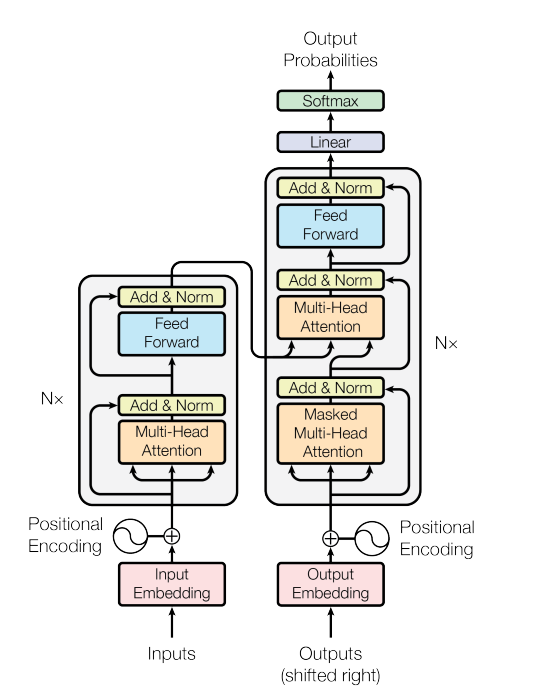
\includegraphics[width=0.5\textwidth]{transformer.png}
  \caption{Transformer - model architectuur \autocite{VaswaniEtAl2017}}
  \label{fig:transformer-model}
\end{figure}


\subsection{Bestaande LLMs}
\label{sec:bestaande-llms}

\subsection{Beperkingen van LLMs}
\label{sec:beperkingen-van-llms}


Door deze nieuwe neurale netwerken zijn er krachtige LLMs ontstaan zoals: GPT van OpenAi  \autocite{RandfordEtAL2018} en BERT van \textcite{DevlinEtAl2019}.
Meta heeft verschillende LLMs waaronder ook 'Code LLama - Python' een LLM speciaal getraind op Python code, deze kan gebruikt worden om documentatie te genereren. \autocite{Roziere2024}
GPT-4 van OpenAi 
%verder aan vullen met verschillende LLMs dieper op in gaan!!



\section{LLM voor documentatie}
\label{sec:llm-voor-documentatie}

Door de kracht van LLMs is het mogelijk om documentatie te genereren. Door de code aan een LLM te geven als input met extra prompts kan de LLM weten wat de code doet.
Deze output kan dan gebruikt worden als verdere input voor de LLM om een samenvatting te genereren van het gehele project.

\section*{{Huidige Python documentatie tools}}
\label{sec:huidige-tools}

Er bestaan reeds verschillende tool waar Python documentatie gegenereerd wordt. De documentatie wordt gegenereerd in verschillende vormen. 
Documentatie aan de hand van docstrings of een API documentatie die de gehele structuur van een Python project volgt. 
Ook is er de mogelijkheid om documentatie te verkrijgen in de vorm van man pages, pdf of in tekstvorm.

Wat zijn docstrings? Docstrings zijn strings die aan het begin van een module, functie, klasse of methode staan. 
En uitleg geven over de werking van de code en wat de uitvoer is.
Docstrings kunnen op verschillende wijzen gegenereerd worden. Zoals het gebruiken van GPT4 \textcite{OpenAI2023} dit werd gedaan door \textcite{Trofficus2023}.

\textcite{Sphinx2023} is een van de meest gebruikte tools voor het genereren van documentatie voor Python projecten.
Sphinx doet dit aan de hand van docstrings. Ook gebruikt het de hierarchie van het project om een duidelijk overzicht te geven van de structuur van het project.
De tool kan met verschillende extensies uitgebreid worden zodat het de juiste functionaliteit heeft voor alle mogelijke wensen.

Pdoc een tool van \textcite{GallantHils2023} genereert een website wat een API van de documentatie bevat. 
Alle functies van het python project kunnen hier makkelijk teruggevonden worden.